%!TEX root = ../../common/main.tex

\chapter{Flavour Tagging}
\label{ch:flavour_tagging}

The time-dependent measurement of the $\CP$ asymmetry $\CPAsymmetry$ in the
decay of $\Bd$ and $\Bdbar$ mesons into the $\CP$ eigenstate $\Jpsi\KS$ requires
the knowledge of the \Bmeson flavour at production, \ie weather it contained
a $\bquark$ or a $\bquarkbar$. The method and algorithms used to infer this
information from all available event properties are named \enquote{flavour
tagging}.

Each tagging algorithm provides a tag $\tagdecision$ and a probability estimate
$\mistagestimate$ that the assigned tag is wrong, also called \enquote{mistag}
estimate. The tag is $\tagdecision=+1$ for an initial $\Bd$, $\tagdecision=-1$
for an initial $\Bdbar$, and $\tagdecision=0$ if the tagging algorithms were not
able to determine a decision. The mistag estimate interval is given by
$[0,0.5[$, where mistags $\mistagestimate^{\prime}>0.5$ are evaluated as
$\mistagestimate = 1 - \mistagestimate^{\prime}$ and the corresponding tag's
sign is reversed. If the algorithm is not able to determine a decision, the
mistag is set $\mistagestimate=0.5$.

The performance of the flavour tagging algorithms can be assigned using control
samples of \Bmesons whose final state determines the $\B$ flavour at decay
time (\ie are \enquote{flavour specific}), \eg $\BuToJpsiK$ where the charge of
the kaon allows to infer the charge of the $\B$.

Given the numbers of all right tagged $\B$ candidates $\NRtagged$, all wrong
tagged candidates $\NWtagged$, and all \enquote{untagged} candidates
$\NUtagged$, the \enquote{tagging efficiency} $\tageff$ can be assigned
%
\begin{equation}\label{eq:flavour_tagging:tageff}
  \tageff = \frac{\NRtagged + \NWtagged}{\NRtagged + \NWtagged + \NUtagged}\eqpd
\end{equation}
%
In addition to the mistag estimate, the true underlying fraction of wrong tagged
candidates $\mistag$ is given by
%
\begin{equation}\label{eq:flavour_tagging:mistag}
  \mistag = \frac{\NWtagged}{\NRtagged + \NWtagged}\eqpd
\end{equation}
%
The statistically relevant \acl{FoM} for time-dependent measurements of $\CP$
violation\addref{for $\efftageff$ for CPV measurements}, the \enquote{effective
tagging efficiency}
%
\begin{equation}\label{eq:flavour_tagging:efftageff}
  \efftageff = \tageff(1 - 2 \mistag)^2 = \tageff \tagdilution^2 \eqcm
\end{equation}
%
represents the fraction of candidates necessary to reach the same statistical
power if the tagging would be perfect, and hence should be maximized to achieve
the best performance. The quantity $\tagdilution$ is called \enquote{dilution},
taking a value of $1$ in case of perfect tagging, and $0$ in case of random
tagging. As described in \cref{missing} the dilution can be directly translated
to the amplitude of the measured $\CP$ asymmetry. \missing{Effect of dilution on CPV asymmetry}

In the following sections more details of the flavour tagging are provided. A
short introduction of the utilized algorithms and a comparison to the flavour
tagging used at lepton colliders is given in \cref{sec:flavour_tagging:lhcb}.
\Cref{sec:flavour_tagging:os,sec:flavour_tagging:ss} describe the two different
classes of flavour tagging algorithms used at \LHCb, while the calibration of
the tagging algorithms outputs is described in
\cref{sec:flavour_tagging:calibration}. The combination of different algorithm
responses into a single decision is outlined in
\cref{sec:flavour_tagging:combination}. Performance numbers are provided in
\cref{sec:flavour_tagging:performance}, recent developments are discussed in
\cref{sec:flavour_tagging:developments}, and finally the experimental impact of
the flavour tagging on the measurement of $\CP$ violation in $\BdToJpsiKS$
decays is provided in \cref{sec:flavour_tagging:sin2beta}.

More details on the flavour tagging used by \LHCb can be found in
\cite{Aaij:2012mu}.

\section{Flavour tagging algorithms}
\label{sec:flavour_tagging:lhcb}

Several tagging algorithms, each specialized on different characteristics of the
underlying event, are used in order to determine the \Bmeson flavour at
production. The algorithms can be classified into two types: the \SS tagging and
\OS tagging algorithms, also called \SS/\OS taggers. The \SS taggers infer the
production flavour of the signal \Bmeson by identifying charged candidates
that have a high chance of being remnants of its hadronisation process. On the
other hand, the \OS taggers exploit the dominant production of \Bmesons
through $\bbbar$ quark pair production, allowing to partially reconstruct the
\bhadron produced together with each reconstructed signal \Bmeson and
thereby infer its initial flavour. \Cref{fig:flavour_tagging:lhcb:schematics}
gives an overview of the tagging algorithms used on the \acl{OS} and \acl{SS}.

The tagging algorithms are developed and trained using simulated $\BuToJpsiK$
and $\BdToDstarmunu$ decays. In an iterative procedure the selection criteria
were optimized in order to maximise the effective tagging efficiency
$\efftageff$. The algorithms only consider charged tracks with a good quality
of the track fit and momenta above $\SI{2}{\GeVc}$. Tracks with a polar angle of
less than $\SI{12}{\mrad}$ with respect to the beamline are declined. Further
on, particles originating from the signal candidate are suppressed by rejecting
all tracks that lie inside a cone of $\SI{5}{\mrad}$ around any signal $\B$
meson daughter. Using \IP requirements tracks from other \acp{PV} are
eliminated.

\Cref{sec:flavour_tagging:os,sec:flavour_tagging:ss} contain detailed
description of the \OS and \SS tagging algorithms. Recent developments that
exceed the scope of the analysis presented in this thesis but will be relevant
in the future are discussed in \cref{sec:flavour_tagging:developments}. Before
coming to the detailed description of the \LHCb flavour tagging algorithms, a
summary of the flavour tagging methods developed at \Babar and \Belle is given.

\begin{figure}
\centering
%!TEX root = ../../../common/main.tex

% Colours 
\definecolor{fcdOrnA}{HTML}{331605}
\definecolor{fcdOrnB}{HTML}{662C0A}
\definecolor{fcdOrnC}{HTML}{99420F}
\definecolor{fcdOrnD}{HTML}{CC5814}
\definecolor{fcdOrnE}{HTML}{FF6E19}
\definecolor{fcdOrnF}{HTML}{FF975B}
\definecolor{fcdOrnG}{HTML}{FFAC7C}
\definecolor{fcdOrnH}{HTML}{FFC19C}
\definecolor{fcdOrnI}{HTML}{FFD6BD}
\definecolor{fcdOrnJ}{HTML}{FFEADE}
\definecolor{fcdBluA}{HTML}{052A33}
\definecolor{fcdBluB}{HTML}{0A5466}
\definecolor{fcdBluC}{HTML}{0F7E99}
\definecolor{fcdBluD}{HTML}{14A8CC}
\definecolor{fcdBluE}{HTML}{19D2FF}
\definecolor{fcdBluF}{HTML}{5BDFFF}
\definecolor{fcdBluG}{HTML}{7CE5FF}
\definecolor{fcdBluH}{HTML}{9CECFF}
\definecolor{fcdBluI}{HTML}{9CECFF}
\definecolor{fcdBluJ}{HTML}{DEF9FF}
\definecolor{fcdGrnA}{HTML}{243304}
\definecolor{fcdGrnB}{HTML}{476608}
\definecolor{fcdGrnC}{HTML}{6B990D}
\definecolor{fcdGrnD}{HTML}{A0E02D}
\definecolor{fcdGrnE}{HTML}{B2FF15}
\definecolor{fcdGrnF}{HTML}{C8FF58}
\definecolor{fcdGrnG}{HTML}{D3FF79}
\definecolor{fcdGrnH}{HTML}{DEFF9B}
\definecolor{fcdGrnI}{HTML}{E9FFBC}
\definecolor{fcdGrnJ}{HTML}{F4FFDE}
\definecolor{fcdVltA}{HTML}{310433}
\definecolor{fcdVltB}{HTML}{620866}
\definecolor{fcdVltC}{HTML}{930D99}
\definecolor{fcdVltD}{HTML}{C411CC}
\definecolor{fcdVltE}{HTML}{F514FF}
\definecolor{fcdVltF}{HTML}{F858FF}
\definecolor{fcdVltG}{HTML}{F979FF}
\definecolor{fcdVltH}{HTML}{FB9BFF}
\definecolor{fcdVltI}{HTML}{FCBCFF}
\definecolor{fcdVltJ}{HTML}{FEDDFF}

\definecolor{fcdGrayA}{HTML}{111111}
\definecolor{fcdGrayB}{HTML}{222222}
\definecolor{fcdGrayC}{HTML}{333333}
\definecolor{fcdGrayD}{HTML}{444444}
\definecolor{fcdGrayE}{HTML}{555555}
\definecolor{fcdGrayF}{HTML}{666666}
\definecolor{fcdGrayG}{HTML}{777777}
\definecolor{fcdGrayH}{HTML}{888888}
\definecolor{fcdGrayI}{HTML}{999999}
\definecolor{fcdGrayJ}{HTML}{AAAAAA}
\definecolor{fcdGrayK}{HTML}{BBBBBB}
\definecolor{fcdGrayL}{HTML}{CCCCCC}
\definecolor{fcdGrayM}{HTML}{DDDDDD}
\definecolor{fcdGrayN}{HTML}{EEEEEE}

\definecolor{fcdTropiteal}    {HTML}{00A8C6}
\definecolor{fcdTealDrop}     {HTML}{40C0CB}
\definecolor{fcdWhiteTrash}   {HTML}{F9F2E7}
\definecolor{fcdAtomicBikini} {HTML}{AEE239}
\definecolor{fcdFeebleWeek}   {HTML}{8FBE00}





\colorlet{ClrTxt}{black}
\colorlet{ClrTxtVeryDarkGray}{fcdGrayE}
\colorlet{ClrTxtDarkGray}{fcdGrayJ}
\colorlet{ClrVtxGray}{fcdGrayM}

\colorlet{ClrSigQuark}{fcdTealDrop}
\colorlet{ClrSigMeson}{fcdTropiteal}
\colorlet{ClrSigArrow}{fcdTropiteal}

\colorlet{ClrTagQuark}{fcdAtomicBikini}
\colorlet{ClrTagMeson}{fcdFeebleWeek}
\colorlet{ClrTagArrow}{fcdFeebleWeek}

\begin{tikzpicture}[
  scale=1, 
  >=stealth',
  font=\small,
  quark_sig/.style={
    align=center, 
    minimum size=3ex,
    circle,
    color=ClrSigQuark,
    fill=ClrSigQuark,
    text=ClrTxt,
    draw, 
    thick,
    inner sep=0pt,
    outer sep=0pt,
    node distance=0ex
  },
  quark_tag/.style={
    align=center, 
    minimum size=3ex,
    circle,
    color=ClrTagQuark,
    fill=ClrTagQuark,
    text=ClrTxt,
    draw, 
    thick,
    inner sep=0pt,
    outer sep=0pt,
    node distance=0ex
  },
  meson_sig/.style={
    draw, 
    align=center, 
    minimum size=4.5ex,
    circle,
    color=ClrSigMeson,
    fill=ClrSigMeson,
    text=ClrTxt,
    thick,
    inner sep=0pt,
    outer sep=1pt,
    node distance=0ex
  },
  meson_tag/.style={
    draw, 
    align=center, 
    minimum size=4.5ex,
    circle,
    color=ClrTagMeson,
    fill=ClrTagMeson,
    text=ClrTxt,
    thick,
    inner sep=0pt,
    outer sep=1pt,
    node distance=0ex
  },
  meson_comb/.style={
    shape=ellipse, 
    draw,
    fill,
    very thick,
    inner sep=0pt,
    outer sep=0pt,
    minimum width=8ex,
    minimum height=5ex},
  vertex/.style={
    shape=ellipse,
    draw,
    inner sep=1ex,
    outer sep=0pt,
    minimum width=10ex,
    minimum height=10ex,
    color=ClrVtxGray,
    fill=ClrVtxGray,
    text=ClrTxt,
    node distance=1ex
  },
  vertex_label/.style={
    inner sep=0pt,
    outer sep=0pt,
    text=ClrTxtDarkGray,
    node distance=1ex,
    font=\sffamily\small
  },
  tagger_label/.style={
    inner sep=0pt,
    outer sep=0pt,
    text=ClrTxtVeryDarkGray,
    node distance=1ex,
    font=\sffamily\small    
  },
  arrow_sig/.style={
    ->,
    very thick,
    color=ClrSigArrow
  },
  arrow_tag/.style={
    ->,
    very thick,
    color=ClrTagArrow
  }
]

%\draw[help lines] (-1,-5) grid (11,5);

\draw[dashed,color=fcdGrayE] (0,0) -- (12,0);
\node[text width=2.5cm,text=ClrTxtDarkGray,font=\sffamily\small] (SST) at (10.5,+0.3) {\hfill same side};
\node[text width=2.5cm,text=ClrTxtDarkGray,font=\sffamily\small] (OST) at (10.5,-0.3) {\hfill opposite side};


\node[draw,circle,fill,color=ClrSigQuark,inner sep=0pt,minimum size=8pt] 
  (coll) at (0,0) {};

\draw[<-,very thick] (coll) -- (+1,0);
\draw[->,very thick] (-1,0) -- (coll);

\begin{pgfonlayer}{foreground}
  
  % bbbar
  \node[quark_sig] (qrk_bbar) at (0.2,+0.8) {$\bquarkbar$};
  \node[quark_sig] (qrk_b) at (0.2,-0.8) {$\bquark$};
  
  \path (qrk_bbar) 
        to[circle connection bar switch color=from (ClrSigQuark) to (ClrSigQuark)] 
        (coll);
  \path (qrk_b) 
        to[circle connection bar switch color=from (ClrSigQuark) to (ClrSigQuark)] 
        (coll);
  
  % Signal decay
  \node[meson_sig,color=ClrSigMeson,fill=ClrSigMeson,text=ClrTxt] (SigJpsi) at (7.5,+2.25) {$\Jpsi$}  ;
  \node[meson_sig,color=ClrSigMeson,fill=ClrSigMeson,text=ClrTxt] (SigKS) [below=of SigJpsi] {$\KS$}  ;
  
  % SS tagging
  \path (qrk_bbar) ++(15:3ex) node (qrk_d) [quark_tag] {$\dquark$};
  
  \node[quark_tag] (qrk_dbar) at (0.8,+2.2) {$\dquarkbar$};
  
  \node[draw,circle,fill,color=ClrTagQuark,inner sep=0pt,minimum size=4pt] 
    (vacuumexc) at ([xshift=-2ex] $(qrk_dbar)!0.5!(qrk_d)$) {};
  
  \path (qrk_d) 
        to[circle connection bar switch color=from (ClrTagQuark) to (ClrTagQuark)] 
        (vacuumexc);
  \path (qrk_dbar) 
        to[circle connection bar switch color=from (ClrTagQuark) to (ClrTagQuark)] 
        (vacuumexc);  
  \path (qrk_dbar) ++(165:3ex) node (qrk_u)    [quark_tag] {$\uquark$};

  \node[meson_tag] (SSpip) at (3.3,+2.7) {$\pip$}; 
  

  % OS tagging
  \path (qrk_b)    ++(-15:3ex) node (qrk_xbar) [quark_tag] {$\quarkbar$};  

  % Tagging particles 
  \node[meson_tag] (OSlepton) at (9.5,-2.25) {$\lepm$};
  \node[meson_tag] (OSkaon)   at (9.5,-1)    {$\Kp$};
  
\end{pgfonlayer} 
  
  
\node[meson_comb,rotate=+15,color=ClrSigMeson,text=ClrTxt] (SigBz) at ($(qrk_bbar)!0.5!(qrk_d)$) {  }; 
\node[meson_comb,rotate=-15,color=ClrTagMeson,text=ClrTxt] (Hb) at ($(qrk_b)!0.5!(qrk_xbar)$) {}; 
\node[meson_comb,rotate=-15,color=ClrTagMeson,text=ClrTxt] (pip_SS) at ($(qrk_dbar)!0.5!(qrk_u)$)   {}; 

  
\begin{pgfonlayer}{background}
  \node[vertex,fit=(SigBz)(Hb)(pip_SS),minimum width=16ex] (PV) {};
  \node[vertex_label,align=center] (PV_label) [above=of PV] {PV};
  
  \node[vertex,fit=(SigJpsi)(SigKS)   ,minimum width=10ex] (SigSV) {};
  \node[vertex_label,align=center] (SigSV_label) [above=of SigSV] {SV};
  
  \node[vertex,minimum width=11ex,minimum height=9ex,align=left] (OS_SV) at (4.5,-1.75) {$\bquark \to \cquark$\\  $\bquark \to X \lepm$};
  \node[vertex_label,align=center] (OS_SV_label) [above=of OS_SV] {SV};
  
  
  \node[vertex,minimum width=9ex,minimum height=7ex,align=center] (OS_TV) at (7.5,-1.25) {$\cquark \to \squark$};
\end{pgfonlayer}


\begin{pgfonlayer}{foreground}
  \draw[arrow_sig] (SigBz)  -- node (Bz_label) [above] {$\Bd$} ([xshift=+4pt] SigSV.west);
  \draw[arrow_sig] let \p1 =(SigJpsi.east) in (\x1-1,\y1+2)  -- (\x1+50,\y1+5);
  \draw[arrow_sig] let \p1 =(SigJpsi.east) in (\x1-1,\y1-2)  -- (\x1+50,\y1-5);
  \draw[arrow_sig] let \p1 =(SigKS.east)   in (\x1-1,\y1+2)  -- (\x1+50,\y1+5);
  \draw[arrow_sig] let \p1 =(SigKS.east)   in (\x1-1,\y1-2)  -- (\x1+50,\y1-5);
    
  \draw[arrow_tag] (Hb)     -- node (Hb_label) [above] {$\hb$}  ([xshift=+4pt] OS_SV.west);
  \draw[arrow_tag] (OS_SV)  -- ([xshift=+4pt] OS_TV.west);
  \draw[arrow_tag] (OS_SV)  -- ([xshift=+0pt] OSlepton.west);
  \draw[arrow_tag] (OS_TV)  -- ([xshift=+0pt] OSkaon.west);
  \draw[arrow_tag] (pip_SS) -- ([xshift=+0pt] SSpip.west);


  \node[tagger_label,align=left] (SSpip_label) [right=of SSpip] {SS pion};
  \node[tagger_label,align=left] (OSlepton_label) [right=of OSlepton] {OS muon\\ OS electron};
  \node[tagger_label,align=left] (OSkaon_label)   [right=of OSkaon] {OS kaon};
  \node[tagger_label,align=center] (OSVtcCh_label) [below=of OS_SV] {OS vertex charge};

\end{pgfonlayer}

\end{tikzpicture}

\caption{Schematic overview of the used \acs*{OS} and \acs*{SS} tagging
algorithms. \cite{wishahi:2013jt}}
\label{fig:flavour_tagging:lhcb:schematics}
\end{figure}

\subsection*{Flavour tagging at \Babar and \Belle}
\label{sec:flavour_tagging:lhcb:b_factories}
Caused by the different nature of the experimental setup the tagging method used
at \LHCb differs from methods used at the \BFactories. As described in
\cref{sec:lhcb_experiment:detector} the \bhadron production is dominated
by gluon-gluon fusion over a large range of $q^2$ in contrast to the production
at the $\YFourS$ $\bbbar$ resonance as it is the case at the \BFactories. The
following section gives a résumé of the flavour tagging methods employed by the
\Babar and \Belle collaborations outlined in \Ref~\cite[][Ch. 8]{Bevan:2014iga}.
%
\begin{figure}
\centering
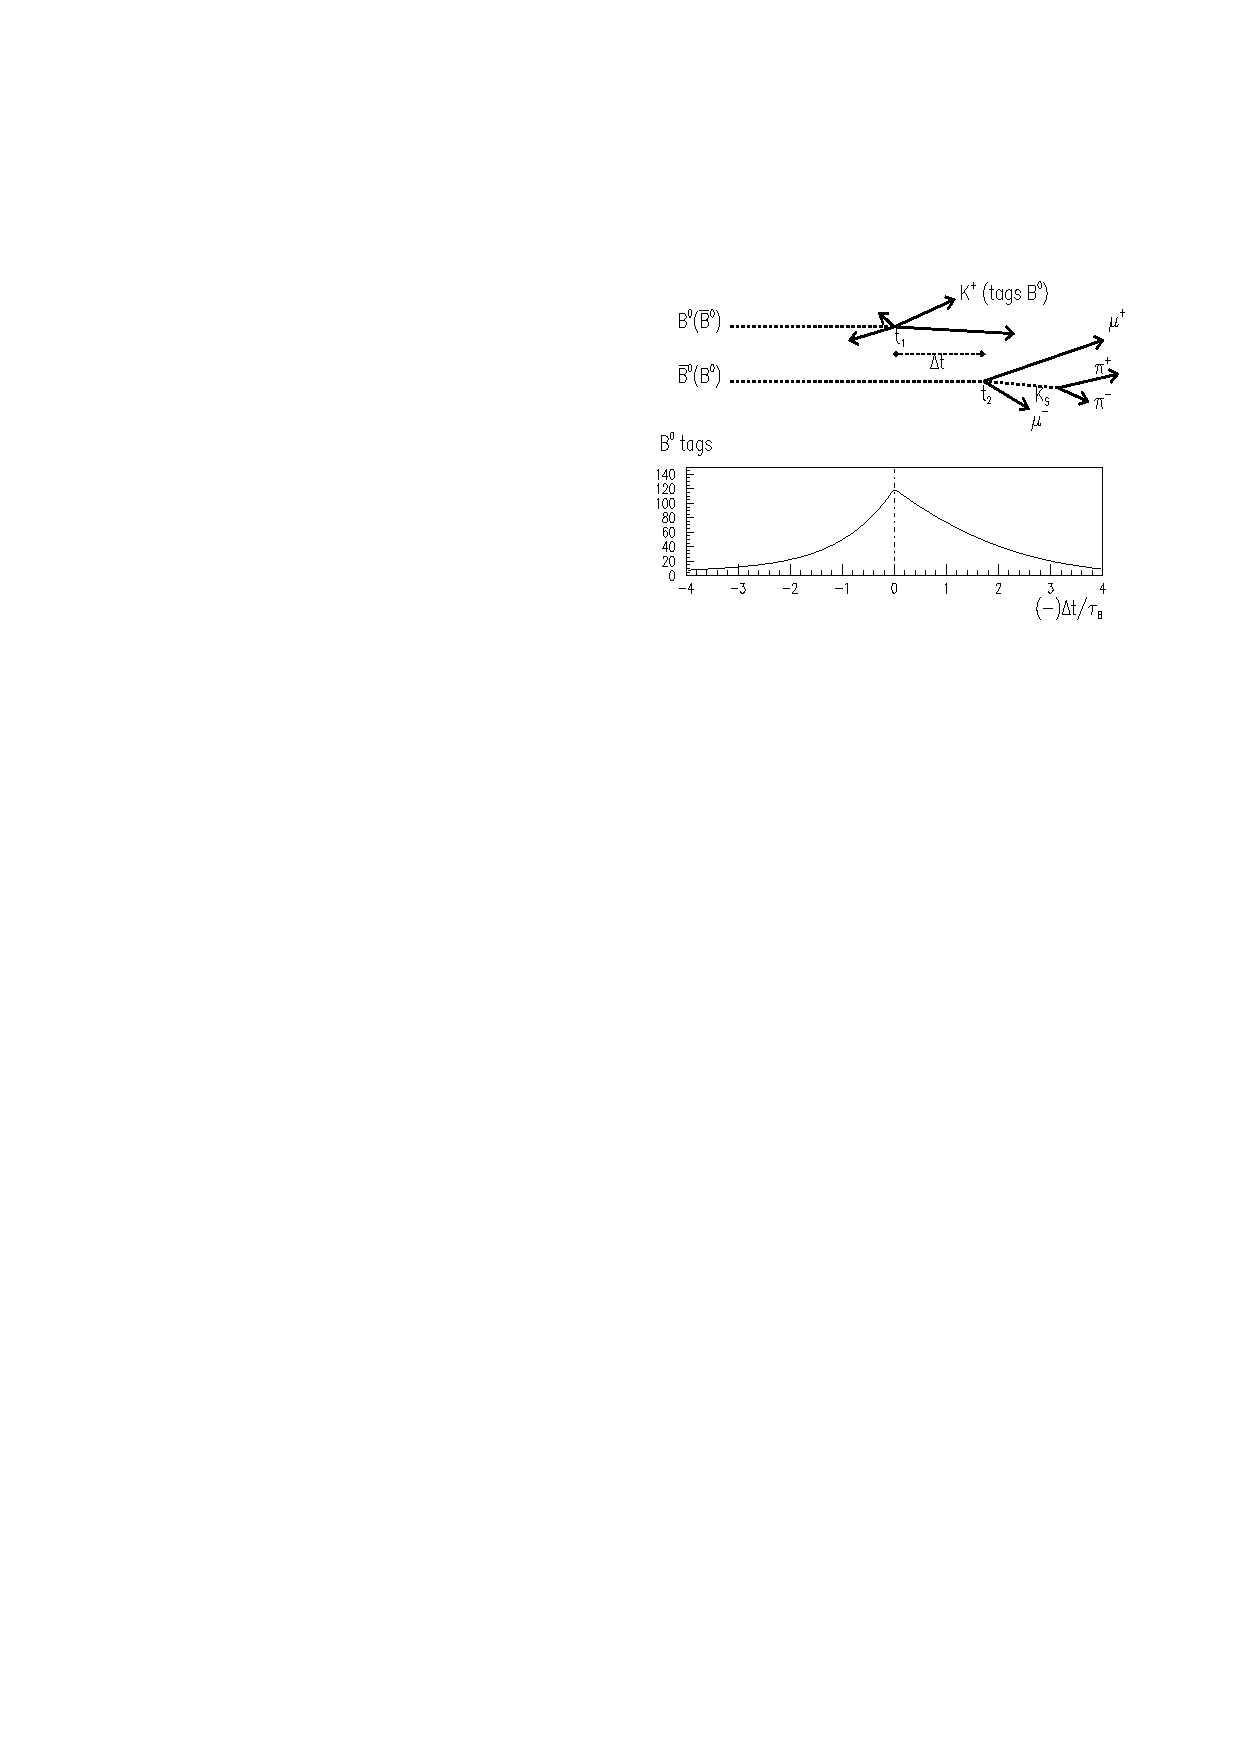
\includegraphics[width=\textwidth]{private/content/flavour-tagging/figs/b_factory_basic_principles}
\caption{Illustration of the measurement of \sintwobeta as conducted by the
\BFactories. \cite{Bevan:2014iga}}
\label{fig:flavour_tagging:lhcb:b_factory_basic_principles}
\end{figure}

\Cref{fig:flavour_tagging:lhcb:b_factory_basic_principles} illustrates the basic
principles of a \CP violation measurement at the \BFactories. The produced
$\Bd\Bdbar$ pair's wave function is in a $P$-wave entangled state, until one of
the mesons decays. From this point in space time ($t_1$) the second $\B$ meson
propagates further through the detector, mixes to its antimatter state, and
finally decays at $t_2$. The \CP asymmetry $\CPAsymmetry$ will therefore be a
function of the decay time difference $\Delta t$. This has two implications:
First, the decay time difference will always be computed relative to the
\enquote{tagging} \Bmeson decay and thus might be negative if the signal $\B$
meson decays first. Secondly, if the tagging \Bmeson decays into a
flavour-specific final state, this specifies the signal \Bmeson's flavour at
$\Delta t=0$.

As a result of the production mechanism, the fully reconstructed signal decay
leaves all remaining tracks to originate from the tagging $\B$. This allows to
classify the decay of the tagging meson according to the signature of the final
state particles. Specialised taggers then identify decays based on their
specific signature. In a second stage, all results provided by the single
taggers are combined into a final tagging decision. 

The lepton taggers deduce a tag from the charge of electrons and muons from
$\bquark \to \cquark \lepm \neutrinobar$ transitions in semileptonic $\B$
decays. Likewise, second order transitions from $\bquark \to \Wm \cquark ( \to
\squark \lepp \neutrino )$ can be used, but has to be handled differently as
their charge is opposite compared to primary leptons. Charged kaon candidates
from the $\bquark \to \cquark \to \squark$ decay chain reflect the charge of the
tagging meson. Here as well, kaons from second order transitions carry the
opposite charge. Charged pions from charm decays work as tagging particles
either directly or in events with both a pion and a charged kaon, the
correlation of the particles can be utilised to improve the tag decision.
Selecting high momentum particles, \eg fast pions from $\Bdbar \to \Dstarp
\pim$, is on its own another source of tagging information and might
additionally be correlated with slow particles to enhance the tagging result.
Finally the flavour of $\Lambda$ baryons from decays of the tagging $\B$ meson
can be exploited.

The \Babar experiment uses \acp{ANN} for each single tagger to provide several
intermediate tagging decisions that are subsequently combined using another \ANN
to gain a joined tagging decision. The effective tagging efficiency of the final
\Babar tagging algorithm is estimated on data to be $\efftageff = \SI{33.1 +-
0.3}{\percent}$. In \Belle analyses the flavour tagging approach is similar.
Instead of \acp{ANN} multi-dimensional look-up tables are used. At first,
information from charged tracks are looked-up to sort them into the signature
categories. Next, the received results are used on an event-level to provide the
final tagging decision. Using this approach an effective tagging efficiency of
$\efftageff = \SI{30.1 +- 0.4}{\percent}$ is achieved.

\subsection{\Acl{OS} algorithms}
\label{sec:flavour_tagging:os}
The \OS algorithms all infer the tagging decision from the quark flavour of the
\bhadron produced in association with the signal \Bmeson. If for
example a $\Bu$ decays into the $\Jpsi\Kp$ final state trough a $\bquarkbar \to
\Wm (\to \cquark \squarkbar) \cquarkbar$ transition, it can unambiguously stated
by looking at the kaon charge that the \bhadron produced along with the $\Bu$
contained a $\bquark$ quark. The tag identification for events with this
signature fall into the scope of the \OSK tagger.
\important{Kaon tagging transition is wrong!}

In total four distinct \OS taggers, each developed for a special \OS decay
signature, provide tagging information. Besides the \OSK tagger, the \OSe and
the \OSm select leptons coming from the primary $\bquark \to X \lepm$ decay to
use their charge as an information carrier of the $\B$ flavour. Finally, the
\OSvtx tagger performs an inclusive reconstruction of the \OS \SV to then
compute a weighted sum of all particle track charges that originate from the
\SV. In the following the selection criteria and algorithms of the \OS taggers
are briefly described.

\missing{Intrinsic mistag due to neutral B meson oscillation}
 
\subsubsection{The \acl{OSK} tagger}
\label{sec:flavour_tagging:os:kaon}
The kaon tagger exploits the charge of kaons stemming from $\bquark \to
\cquark \to \squark$ decays of opposite side \bhadrons. As the charge of the
kaon is the opposite of the ancestor's charge, the kaon always carries the same
charge as the signal \Bmeson.

To reduce background contributions of prompt kaons and kaons from primary
$\bquarkbar \to \Wm (\to \cquark \squarkbar) \cquarkbar$ transitions, in which
case the kaon carries the \enquote{wrong} charge, several selection criteria are
applied. Cuts on the \pT, the \IP, the \IP/$\sigma_\text{\IP}$, and the track
fit $\chi^2/\ndf$ are performed. \PID requirements on the \DLLKpi, the \DLLppi,
and \DLLmupi suppress mis-identified particles. Clone tracks are removed and
kaon candidates with originate from other \acp{PV} are rejected using a cut on
the \IP/$\sigma_\text{\IP}$ with respect to any \PV. \cref{tab:} lists all
applied cuts.
\missing{Table with cut values}

K charge is the same as signal B (opposite if K not from b->c->s but from bcW->s)
K pT>0.5, IP<1.25mm, IP/error>3.35, track chi2/ndf<2.75
suppress prompt kaons
PID DLLkπ > 6
(DLLkπ - DLLpπ) > -4
remove clone tracks (Kullback-Liebler criterion)
additional pile-up PV cut of IP/sigma > 4.5
if more than one candidate, highest pT
only Probkaon>0.54
How to suppress bcW->s kaons?

\subsubsection{The \acl{OSe} and the \acl{OSm} taggers}
\label{sec:flavour_tagging:os:lepton}
leptons from bcW->leptons
lepton charge, same as signal b
muons:
DDLmuπ>1
track chi2/ndf<3.2
pT>1.2GeV to reduce b->c->mu secondary muons
reduce fake muons "non shared hits"
clone tracks

electrons:
DLLeπ>4
HCAL acceptance
pT>1.2GeV
max ionisation charge in VELO (reduce background due to photon conversion close to interaction point)
partial energy E in emCalo
p from tracking system
==> E/p>0.8

highest pT lepton

\subsubsection{The \acl{OSvtx} tagger}
\label{sec:flavour_tagging:os:vertex}
inclusive reco of OS SV:

Summary:
2-track seed from all possible track candidate pairs
geometric and kinematical cuts, then add more tracks
weighted charge of SV
cuts on SV to optimize epseff

Detailed:
2-track seed track selection:
one of the tracks must be a long track w/ track fit chi2/ndf<2.5
error on IP on PV < 1 (no badly reconstructed tracks)
no tracks from PV: IP on PV/error in range 2.5-100
IP on PV < 3mm   ???
pT > 0.15GeV
at least one track pT > 0.3GeV
the two tracks must be separated in phi by more than 1mrad

vertex fit for track pairs:
fit succeeds and chi2/ndf<10 consider pair V as seed

seed requirements:
forward direction from PV (z>0)
detector acceptance
r-distance       ???
seed invariant mass > 0.2 GeV
reject if invariant mass = KS mass

likelihood for all possible seeds based on:
vertex fit chi2/ndf
minimum pT
maximum PV IP 
minimum PV IP/error of both tracks
delta phi 
r-distance
angle between seed direction wrt the PV

seed with maximum likelihood
if likelihood is > 0.6

algorithm is nearly 50percent efficient
60percent of seed track pairs from b hadron decay

adding more tracks from the tagging tracks to the seed if:
no clone track
track chi2/ndf < 3
PV IP > 0.1mm
PV IP/error > 3.5
seed IP < 0.9mm
DOCA to any track in seed < 0.2mm

60 percent of added tracks come from b hadron decay

weighted charge of tracks

$Q = \frac{\sum_i \pT^k(i)Q_i}{\sum_i\pT^k(i)}$

k parameter optimized to 0.4
Q<0.25 set to untagged

additional cuts on the SV properties to optimize epseff:
sum of SV track momenta > 10GeV
and invariant SV mass > 0.5GeV
pT sum of all SV tracks > 10 GeV
IP sum SV /error > 10
DOCA sum SV < 0.5mm
only events that satisfy these requirements are considered.

Only use vtx Q if the minimal probability of the tagger to be correct is larger 0.54

\newpage

\subsection{\Acl{SS} algorithms}
\label{sec:flavour_tagging:ss}
SS algorithms: kaon/pion/proton

\section{Calibration}
\label{sec:flavour_tagging:calibration}
\begin{itemize}
  \item calibration method
  \item tagging correlations
  \item OS calibration using Bu2JpsiK: procedure, transferability/validity to Bd2JpsiKS
  \item SS calibration using Bd2JpsiKst: procedure, transferability/validity to Bd2JpsiKS
  \item determination of systematic uncertainties
\end{itemize}
\subsection{OS calibration using Bu2JpsiK}
\label{sec:flavour_tagging:calibration:os}
\subsection{SS calibration using Bd2JpsiKst}
\label{sec:flavour_tagging:calibration:ss}

\section{Combination}
\label{sec:flavour_tagging:combination}
Combination of OS and SS tagging, FT correlations

\section{Performance}
\label{sec:flavour_tagging:performance}
Performance of the FT algorithms, effect on dilution of asymmetry
influence on measuring sin2beta, Dilution

\section{Recent developments}
\label{sec:flavour_tagging:developments}

\section{Influence on the measurement of sin2beta}
\label{sec:flavour_tagging:sin2beta}
